\documentclass[APA,LATO1COL]{WileyNJD-v2}
\usepackage{lmodern}

\articletype{Article Type}%

\received{26 April 2023}
\revised{6 June 2023}
\accepted{6 June 2023}

\raggedbottom


\begin{document}


\title{Case-Base Neural Networks: survival analysis with time-varying,
higher-order interactions}

\author[1]{Jesse Islam}

\author[2]{Maxime Turgeon}

\author[3]{Robert Sladek}

\author[4]{Sahir Bhatnagar}



\address[1]{\orgdiv{Department of Quantitative life sciences,} \orgname{McGill University}, \orgaddress{\state{Quebec}, \country{Canada}}}

\address[2]{\orgdiv{Department of Statistics}, \orgname{University of Manitoba}, \orgaddress{\state{Manitoba}, \country{Canada}}}

\address[3]{\orgdiv{Department of Human Genetics}, \orgname{McGill University}, \orgaddress{\state{Quebec}, \country{Canada}}}

\address[4]{\orgdiv{Department of Biostatistics}, \orgname{McGill University}, \orgaddress{\state{Quebec}, \country{Canada}}}

\corres{Jesse Islam's \email{jesse.islam@mail.mcgill.ca}}

\presentaddress{McGill genome center: 740 Dr Penfield Ave, Montreal, Quebec H3A 0G1}

\abstract[Summary]{Neural network-based survival methods can model data-driven covariate interactions.
While these methods have led to better predictive performance than regression-based approaches,
they cannot model both time-varying interactions and complex baseline hazards. To address this, we
propose Case-Base Neural Networks (CBNN) as a new approach that combines the case-base sampling
framework with flexible architectures. Our method naturally accounts for censoring and does not require
method specific hyperparameters. Using a novel sampling scheme and data augmentation, we incorporate
time directly into a feed-forward neural network. CBNN predicts the probability of an event occurring at a
given moment to estimate the hazard function. We compare the performance of CBNN to survival methods
based on regression and neural networks in a simulation and three real data applications. We report two time-dependent
metrics for each model. For a complex simulation, which highlights the ability of CBNN to model both a complex
baseline hazard and time-varying interactions and two real data applications, CBNN outperforms all competitors
on a simulation with a complex baseline hazard and time-varying interaction and two case studies. A final case
study shows competitive performance. We highlight the benefit of combining case-base sampling with deep
learning to provide a simple and flexible modeling framework for data-driven, time-varying interaction modeling
of survival outcomes. An R package is available at https://github.com/Jesse-Islam/cbnn.}

\keywords{survival analysis, machine learning, case-base, neural
network}



\maketitle




\hypertarget{introduction}{%
\section{Introduction}\label{introduction}}



Smooth-in-time accelerated failure time (AFT) models can estimate absolute
risks by modeling the hazard directly through a user-specified baseline hazard
distribution \citep{kleinbaum2012survival}. Analysts use Cox proportional hazards
models more often than AFT models \citep{hanley2009}. This preference causes
analyses to be based on hazard ratios and relative risks rather than on survival
curves and absolute risks \citep{hanley2009}. With AFT models, it may be difficult
to identify an appropriate baseline hazard for common diseases with many
interacting risk factors \citep{royston2002flexible}. In studies where the disease
pathogenesis may change with age, we may see non-proportional hazards
\citep{coradini2000time}. For example, previous studies of breast cancer incidence
have discovered time-varying interactions with covariates of interest, such as tumor
size \citep{coradini2000time}. One approach to provide flexibility in the baseline hazard
involves using the basis of splines on time in the model \citep{royston2002flexible}.
However, regression-based models require prior knowledge of potential time-varying
interactions and their quantitative effects.


Neural networks provide a data-driven approach to approximating interaction terms.
For example, DeepSurv is a neural network-based proportional hazards model that
implements the Cox partial log-likelihood as a custom loss function \citep{katzman2018DeepSurv}.
This results in a stepwise absolute risk curve that cannot accommodate time-varying interactions.
Compared to Cox regression, DeepSurv shows better performance on a real dataset
\citep{katzman2018DeepSurv}. Previous work suggests we may change the loss function
to address non-proportional hazards \citep{faraggi1995neural}.

DeepHit assumes an inverse Gaussian distribution as the baseline hazard \citep{lee2018DeepHit}.
It specifies each follow-up time time of interest in the model and directly estimates survival curves, rather
than deriving a hazard function \citep{lee2018DeepHit}. DeepHit outperformed DeepSurv
\citep{lee2018DeepHit}.

We note that these alternative neural network approaches require custom loss functions
\citep{katzman2018DeepSurv} \citep{lee2018DeepHit}. DeepHit introduces a hyperparameter
weighing its two loss functions (negative log-likelihood and ranking losses) \citep{lee2018DeepHit}.
Regression-based approaches require prior specification of all interaction terms, which makes it
challenging to model covariate effects that change with time. The current neural network models
provide flexibility at the cost of clarity, while regression models provide clarity at the cost of flexibility.

In this article, we propose Case-Base Neural Networks (CBNN) as a method that models time-varying
interactions and a flexible baseline hazard. Our approach to modeling the full hazard uses case-base
sampling \citep{hanley2009}. This sampling technique allows probabilistic models to predict survival
outcomes. After case-base sampling, we can easily implement the model in any language using
common neural network components. As part of the case-base framework, we use transformations
of time as a feature (covariate) to specify different baseline hazards. For example, by including
splines of time as covariates, we can approximate the Royston-Parmar flexible baseline hazard model
\citep{royston2002flexible}\citep{hanley2009}. However, this still requires explicit use of time-varying
interactions. CBNN can model both without extra tuning parameters.

We describe how case-base sampling and neural networks combine
in Section \ref{methods}, along with our hyperparameter selection procedure, metrics and software implementation.
We explore the performance of CBNN, DeepSurv, DeepHit, Cox regression and case-base using logistic
regression (CBLR) on simulated data in Section \ref{sims}. Section \ref{casestudies} describes the
performance of the same methods in three case studies. Section \ref{discussion} explores the
implications of our results and contextualizes them within neural network survival analysis in a
single event setting.



%%%%%%%%%%%%%%%%%%%%%%%%%%%%%%%%%%%%%%%%%%%%%%
%%%%%%%%%%%%%%%%%%%%%%%%%%%%%%%%%%%%%%%%%%%%%%
%%%%%%%%section2
%%%%%%%%%%%%%%%%%%%%%%%%%%%%%%%%%%%%%%%%%%%%%%
%%%%%%%%%%%%%%%%%%%%%%%%%%%%%%%%%%%%%%%%%%%%%%

\hypertarget{methods}{%
\section{Case-base neural networks, metrics, hyperparameters and
software}\label{methods}}

In this section, we define case-base sampling, which converts the total
survival time into discrete person-specific moments (person-moments).
Next, we detail how neural networks can be used within this framework,
explicitly incorporating time as a feature while adjusting for the
sampling bias. Then, we describe the metrics and hyperparameter selection procedure.
Finally, we report on the software versions used. An R
package is available for use at
\url{https://github.com/Jesse-Islam/cbnn}. The entire code base to
reproduce the figures and empirical results in this paper is available
at \url{https://github.com/Jesse-Islam/cbnnManuscript}.

\hypertarget{case-base-sampling}{%
\subsection{Case-base sampling}\label{case-base-sampling}}

Case-base sampling is an alternative framework for survival analysis
\citep{hanley2009}. Without this preliminary step, we cannot model survival
outcomes with probabilistic methods. In case-base sampling, we sample from the continuous
survival time of each person in our dataset to create a \emph{base
series} of \emph{person-moments}. This \emph{base series} complements
the \emph{case series}, which contains all person-moments at which the
event of interest occurs.

For each person-moment sampled, let \(X_i\) be the corresponding
covariate profile \(\left(x_{i1},x_{i2},...,x_{ip} \right)\), \(T_i\) be
the time of the person-moment and \(Y_i\) be the indicator variable for
whether the event of interest occurred at time \(T_i\). We estimate the
hazard function \(h(t \mid X_i)\) using the sampled person-moments.
Recall that \(h(t \mid X_i)\) is the instantaneous potential of
experiencing the event at time \(t\) for a given set of covariates
\(X_i\), assuming \(T_i \geq t\).

Now, let \(b\) be the (user-defined) size of the \emph{base series} and
let \(B\) be the sum of all follow-up times for the individuals in the
study. let $c$ be the number of events in the \emph{case series}.
A reasonable concern is determining how large $b$ should be relative to $c$.
The size of \(b\) influences how much information is lost in the sampling process
\citep{hanley2009}. Using our notation, Hanley $\&$ Miettinen (2009)
adapt a quote from Mantel (1973): "By the reasoning that $\frac{cb}{c+b} [=(\frac{1}{c}+\frac{1}{b}]$
measures the relative information in a comparison of two averages based on
sample sizes of c and b respectively, we might expect by analogy, which would
of course not be exact in the present case, that this approach would result in
only a moderate loss of information. (The practicing statistician is generally
aware of this kind of thing. There is little to be gained by letting the size of
one series, b, become arbitrarily large if the size of the other series, c, must
remain fixed)" \citep{hanley2009} \citep{mantel1}. If $b=100c$, then we expect learned
weights to be at most one percent higher than if the entire study base $B$ was used,
as they are proportional to $\frac{1}{c}+\frac{1}{100c}$ rather than $\frac{1}{c}+\frac{1}{\infty c}$ \citep{hanley2009}.

If we sample the \emph{base series} uniformly across the study
base, then the hazard function of the sampling process is equal to
\(b/B\). Therefore, we have the following equality \cite{saarela2015}
\footnote{We are abusing notation here, conflating hazards with probabilities. For a rigorous treatment, see Saarela \& Hanley (2015) section 3 \cite{saarela2015} .}:
\begin{align}\label{eqn:main}
\frac{P\left(Y_i=1 \mid X_i, T_i\right)}{P\left(Y_i = 0 \mid X_i, T_i\right)} = \frac{h\left(T_i \mid X_i\right)}{b/B}.
\end{align} The odds of a person-moment being a part of the \emph{case
series} is the ratio of the hazard \(h(T_i \mid X_i)\) and the uniform
rate \(b/B\). Using \eqref{eqn:main}, we can see how the log-hazard
function can be estimated from the log-odds arising from case-base
sampling: \begin{align}\label{eqn:offset}
\log \left( h\left(t \mid X_i\right)\right) = \log \left(\frac{P\left(Y_i = 1 \mid X_i, t\right)}{P\left(Y_i = 0 \mid X_i, t\right)}\right) + \log\left(\frac{b}{B}\right).
\end{align}

To estimate the correct hazard function, we adjust for the bias
introduced when sampling a fraction of the study base (\(\frac{b}{B}\)) by adding
the term \(\log\left(\frac{B}{b} \right)\) to offset \(\log\left(\frac{b}{B} \right)\)
during the fitting process. Next, we propose using neural networks to model the
odds.

\hypertarget{neural-networks-to-model-the-hazard-function}{%
\subsection{Neural networks to model the hazard
function}\label{neural-networks-to-model-the-hazard-function}}

After case-base sampling, we pass all features, including time, into any
user-defined feed-forward component, to which an offset term is added,
then passed through a sigmoid activation function (Figure
\ref{fig:NNarch}). We are interested in predicting the odds. This makes the sigmoid
activation function ideal as it is the inverse of the odds. which we can use to calculate the hazard. The general form for the
neural network using CBNN is:

\begin{align*}
P\left(Y=1|X,T\right)&=\mathrm{sigmoid}\left(f_{\theta}(X, T) + \log\left(\frac{B}{b}\right) \right),
\end{align*}

where \(T\) is a random variable representing the event time, \(X\) is
the random variable for a covariate profile, \(f_{\theta}(X, T)\)
represents any feed-forward neural network architecture,
\(\log\left(\frac{B}{b}\right)\) is the offset term for adjust for the bias
(\(\log\left(\frac{b}{B}\right)\)) set by case-base sampling,
\(\theta\) is the set of parameters learned by the neural network and
\(\mathrm{sigmoid}(x)=\frac{1}{1+e^{-x}}\). By approximating a
higher-order polynomial of time using a neural network, the baseline
hazard specification is now data-driven, where user-defined
hyperparameters such as regularization, number of layers and nodes
control the flexibility of the hazard function. We provide a detailed
description of the choices we made in the next sub-section.

\begin{figure}

{\centering 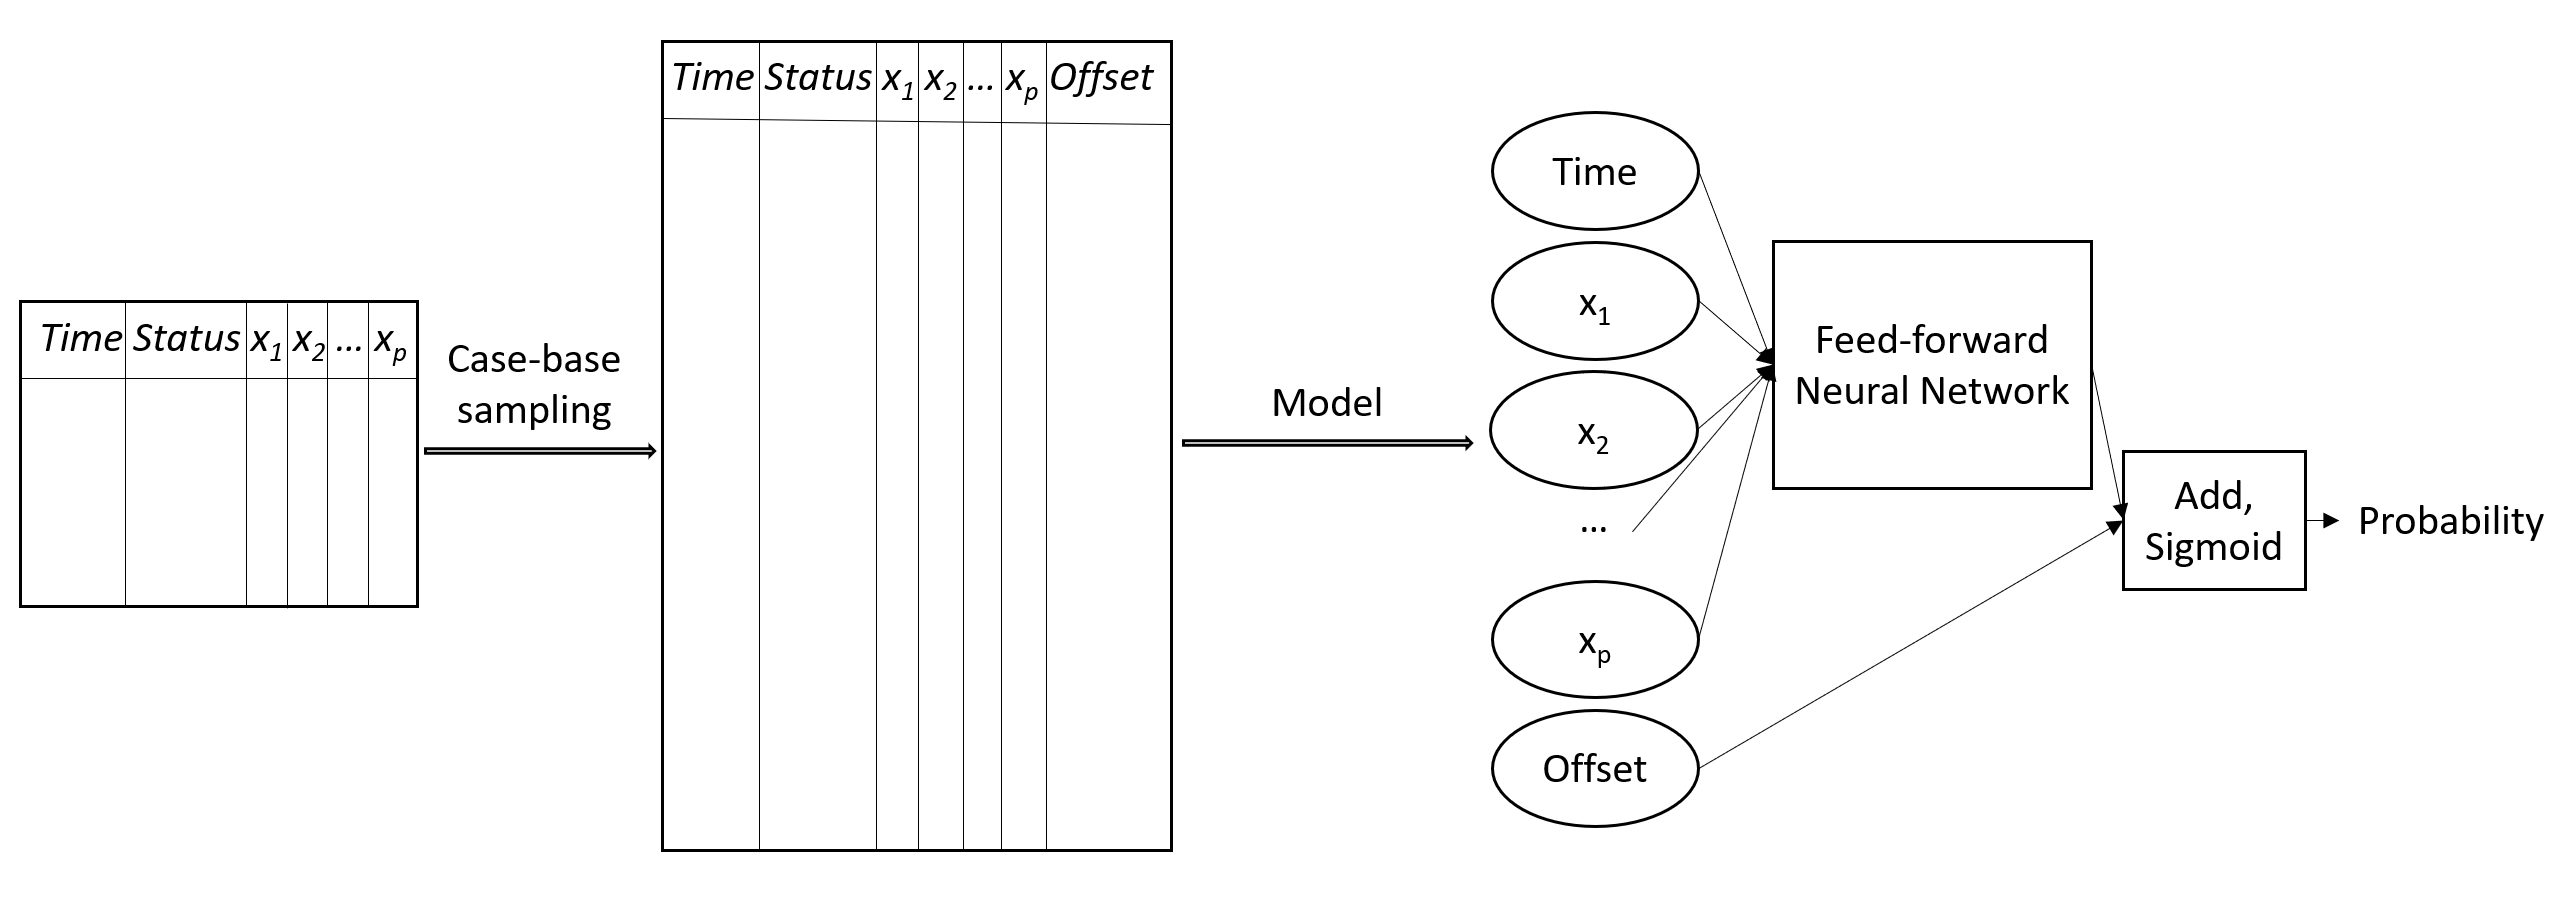
\includegraphics[width=1\linewidth]{../figures/nnarch2}}

\caption{Steps involved in CBNN from case-base sampling to the model framework we use for training. The first step is case-base sampling, completed before training begins. Next, we pass this sampled data through a feed-forward neural network. We add the offset and pass that through a sigmoid activation function, whose output is a probability. Once the neural network model completes its training, we can convert the probability output to a hazard, using it for our survival outcomes of interest.}\label{fig:NNarch}
\end{figure}

The following derivation shows how our probability estimate is converted
to odds: \begin{align*}
 \log\left( h(t \mid X) \right) &= \log\left(\frac{\mathrm{sigmoid}\left(f_{\theta}(X, T) + \log\left(\frac{B}{b}\right)\right)}{1-\mathrm{sigmoid}\left(f_{\theta}(X, T) + \log\left(\frac{B}{b}\right)\right)}\right) + \log\left(\frac{b}{B}\right) \\
 &= \log\left( \frac{\frac{\exp\left(f_{\theta}(X, T) + \log\left(\frac{B}{b}\right)\right)}{\exp\left(f_{\theta}(X, T) + \log\left(\frac{B}{b}\right)\right)+1}}{1-\frac{\exp\left(f_{\theta}(X, T) + \log\left(\frac{B}{b}\right)\right)}{\exp\left(f_{\theta}(X, T) + \log\left(\frac{B}{b}\right)\right)+1}}\right) + \log\left(\frac{b}{B}\right) \\
 &= \log\left(\exp\left( f_{\theta}(X, T) + \log\left(\frac{B}{b}\right) \right) \right) + \log\left(\frac{b}{B}\right) \\
 &= f_{\theta}(X, T) + \log\left(\frac{B}{b}\right) + \log\left(\frac{b}{B}\right) \\
&= f_{\theta}(X, T). 
\end{align*}

We use binary cross-entropy as our loss function \citep{gulli2017}:
\begin{align*}
L(\theta)=-\frac{1}{N} \sum^{N}_{i=1} y_{i} \cdot \log(\hat{f}_{\theta}(x_{i}, t_{i}) ) + (1-y_{i} )\cdot \log(1-\hat{f}_{\theta}(x_{i}, t_{i}) ),
\end{align*} where \(\hat{f}_{\theta}(x_{i}, t_{i})\) is our estimate
for a given covariate profile and time, \(y_{i}\) is our target value
specifying whether an event occurred and \(N\) represents the number of
individuals in our training set.

Backpropagation with an appropriate minimization algorithm (e.g.~Adam,
RMSPropagation, stochastic gradient descent) is used to optimize the
parameters in the model \citep{gulli2017}. For our analysis, we use Adam
as implemented in Keras \citep{gulli2017}. Note that the size of the
\emph{case series} is fixed as the number of events, but we can make the
\emph{base series} as large as we want. A ratio of 100:1 \emph{base
series} to \emph{case series} is sufficient \citep{hanley2009}. We pass
our feed-forward neural network through a sigmoid activation function
(Figure \ref{fig:NNarch}). Finally, we can convert this model output to
a hazard. To use CBNN for predictions, we manually set the
offset term \(\log\left(\frac{B}{b} \right)\) to 0 in the new data as we already account for the bias during the
fitting process.

Since we are directly modeling the hazard, we can readily estimate the
risk function (\(F\)) at time \(t\) for a covariate profile \(X\),
viz.\begin{align}\label{eqn:ci2}
F\left(t\mid X\right)& = 1 - \exp\left(-\int_{0}^{t}h(u|X) \,\textrm du\right).
\end{align} We use a finite Riemann sum \citep{hughes2020calculus} to
approximate the integral in \eqref{eqn:ci2}.



\hypertarget{performance-metrics}{%
\subsection{Performance metrics}\label{performance-metrics}}

To choose our method-specific hyperparameters, we use the Integrated
Brier Score (IBS) \citep{graf1999}. We use two metrics to assess the
performance of the different methods of interest on testing data: 1) Index of Prediction Accuracy (IPA)
\citep{kattan2018index} and 2) Inverse probability censoring weights-adjusted time dependent
area under the receiver operating characteristic curve ($AUC_{IPCW}$) \citep{auc}, which we 
define below. We achieve a summarized assessment of performance for each model with the
IBS. The IPA is a metric for both discrimination and calibration. The $AUC_{IPCW}$
provides a metric for discrimination only. Together, we can get a clearer picture about how
each model performs in each study and why.


\hypertarget{index-of-prediction-accuracy-ipa}{%
\subsubsection{Index of prediction accuracy (IPA)}\label{index-of-prediction-accuracy-ipa}}

The IPA is a function of the Brier score (\(BS(t)\)) \citep{graf1999},
which is defined as \begin{align}\label{eqn:bs}
BS(t)=\frac{1}{N}\sum^{N}_{i=1}\left(\frac{\left(1 - \widehat{F}(t \mid X_{i})\right)^{2}\cdot I(T_{i}\leq t,\delta_{i}=1)}{\widehat{G}(T_{i})} + \frac{\widehat{F}(t\mid X_{i})^{2}\cdot I(T_{i}>t)}{\widehat{G}(t)}\right),
\end{align} where \(\delta_{i}=1\) shows individuals who have
experienced the event, \(N\) represents the number of samples in our
dataset over which we calculate \(BS(t)\), \(\widehat{G}(t)=P[c>t]\) is
a non-parametric estimate of the censoring distribution, \(c\) is
censoring time and \(T_{i}\) is an individual's survival or censoring
time. The BS provides a score that accounts for the information
loss because of censoring. There are three categories of individuals
that may appear within the dataset once we fix our \(t\) of interest.
Individuals who experienced the event before \(t\) are present in the
first term of the equation. The second term of the equation includes
individuals who experience the event or are censored after \(t\). Those
censored before \(t\) are the third category of people. The inverse
probability censoring weights (IPCW) adjustment (\(G(\cdot)\)) is to
account for these category three individuals whose information is
missing. 

The IPA as a function of time is given by \begin{align}
\textrm{IPA}(t) &= 1-\frac{BS_{model}(t)}{BS_{null}(t)}, \nonumber
\end{align} where \(BS_{model}(t)\) represents the BS over time
\(t\) for the model of interest and \(BS_{null}(t)\) represents the
BS if we use an unadjusted Kaplan-Meier (KM) curve as the
prediction for all observations \citep{kattan2018index}. Note that IPA
has an upper bound of one, where positive values show an increase in
performance over the null model and negative values show that the null
model performs better. These scores show how performance changes over
follow-up time. As an extension of BS, IPA models for both calibration
and discrimination\citep{graf1999} \citep{kattan2018index}.

\hypertarget{integrated-brier-score-ibs}{%
\subsubsection{Integrated Brier Score (IBS)}\label{integrated-brier-score-ibs}}

The Integrated Brier Score (IBS) is a function of the BS \ref{eqn:bs} as well \citep{graf1999},
which is defined as \begin{align*}
IBS(t)=\int_{t}^{t_{max}}BS(t)dw(t),
\end{align*} where $w(t)=\frac{t}{t_{max}}$. As this is a score for a range of follow-up-times,
it is a useful metric to track during cross-validation. The performance at a specific time is lost,
and is why we opt for the IPA in assessing performance on a test set.

\hypertarget{auc}{%
\subsubsection{Inverse probability censoring weights-adjusted time dependent area under the receiver operating characteristic curve ($AUC_{IPCW}$) }\label{auc}}

The IPCW-adjusted AUC ($AUC_{IPCW}$) is a time-dependent metric that considers censoring \citep{auc}. 
For a given follow-up time of interest,
 \begin{align*}
AUC_{IPCW}(t)=\frac{\sum^{n}_{i=1}\sum^{n}_{j=1} I \left(\widehat{F}(t|X_{i})>\widehat{F}(t|X_{j})\right) \cdot I(T_{i}\leq t,\delta_{i}=1) \cdot \left( 1-I(T_{j}\leq t,\delta_{j}=1) \right) \cdot W_{i}(t) \cdot W_{j}(t)} { \sum^{n}_{i=1}\sum^{n}_{j=1} I(T_{i}\leq t,\delta_{i}=1) \cdot \left( 1-I(T_{j}\leq t,\delta_{j}=1) \right) \cdot W_{i}(t) \cdot W_{j}(t) },
\end{align*}where \begin{align*}
W_{i}(t)=\frac{I(T_{i}\leq t,\delta_{i}=1)}{\widehat{G}(T_{i})} +\frac{I(T_{i}>t)}{\widehat{G}(t)}.
\end{align*} The $AUC_{IPCW}$ measures discrimination \citep{auc}.
By taking both IPA and $AUC_{IPCW}$ together, we can better understand whether a model is better
in terms of calibration or discrimination.

\hypertarget{hyperparameter-selection}{%
\subsection{Hyperparameter selection}\label{hyperparameter-selection}}

Neural networks are flexible when defining the architecture and optimization parameters.
These hyperparameter choices can affect the estimated parameters and are not necessarily
the same for each model. We apply the same procedure to each study in this paper. First,
we fix a test set with 15\% of the data. We keep aside this data during hyperparameter
selection and we fit a model for each method in each study. To determine the best
hyperparameters for each neural network method, we use three-fold cross-validated grid
search \citep{gulli2017} on the remaining data (85\% training, 15\% validation) for the
following range of hyperparameters:

\[
Grid\ search: \begin{cases}
Learning\ rate \sim \{0.001, 0.01\} \\ %technically a control and treatement group
Dropout \sim \{0.01,0.05, 0.1\} \\
First\ layer\ nodes \sim \{50, 75, 100\} \\
Second\ layer\ nodes \sim \{10,25,50\} \\
Number\ of\ batches \sim \{100, 500\} \\
Activation\ function \sim \{ReLU, Linear\}\\
\alpha \sim \{0, 0.5, 1\}.
\end{cases}
\] 

\begin{table}
\caption{Four tables showing the chosen hyperparameters along with the IBS for each neural network model in the complex simulation (A), multiple myeloma (MM) case study (B), free light chain (FLC) case study (C) and prostate cancer (Prostate) case study (D).}
\label{tab:wins}
\begin{center}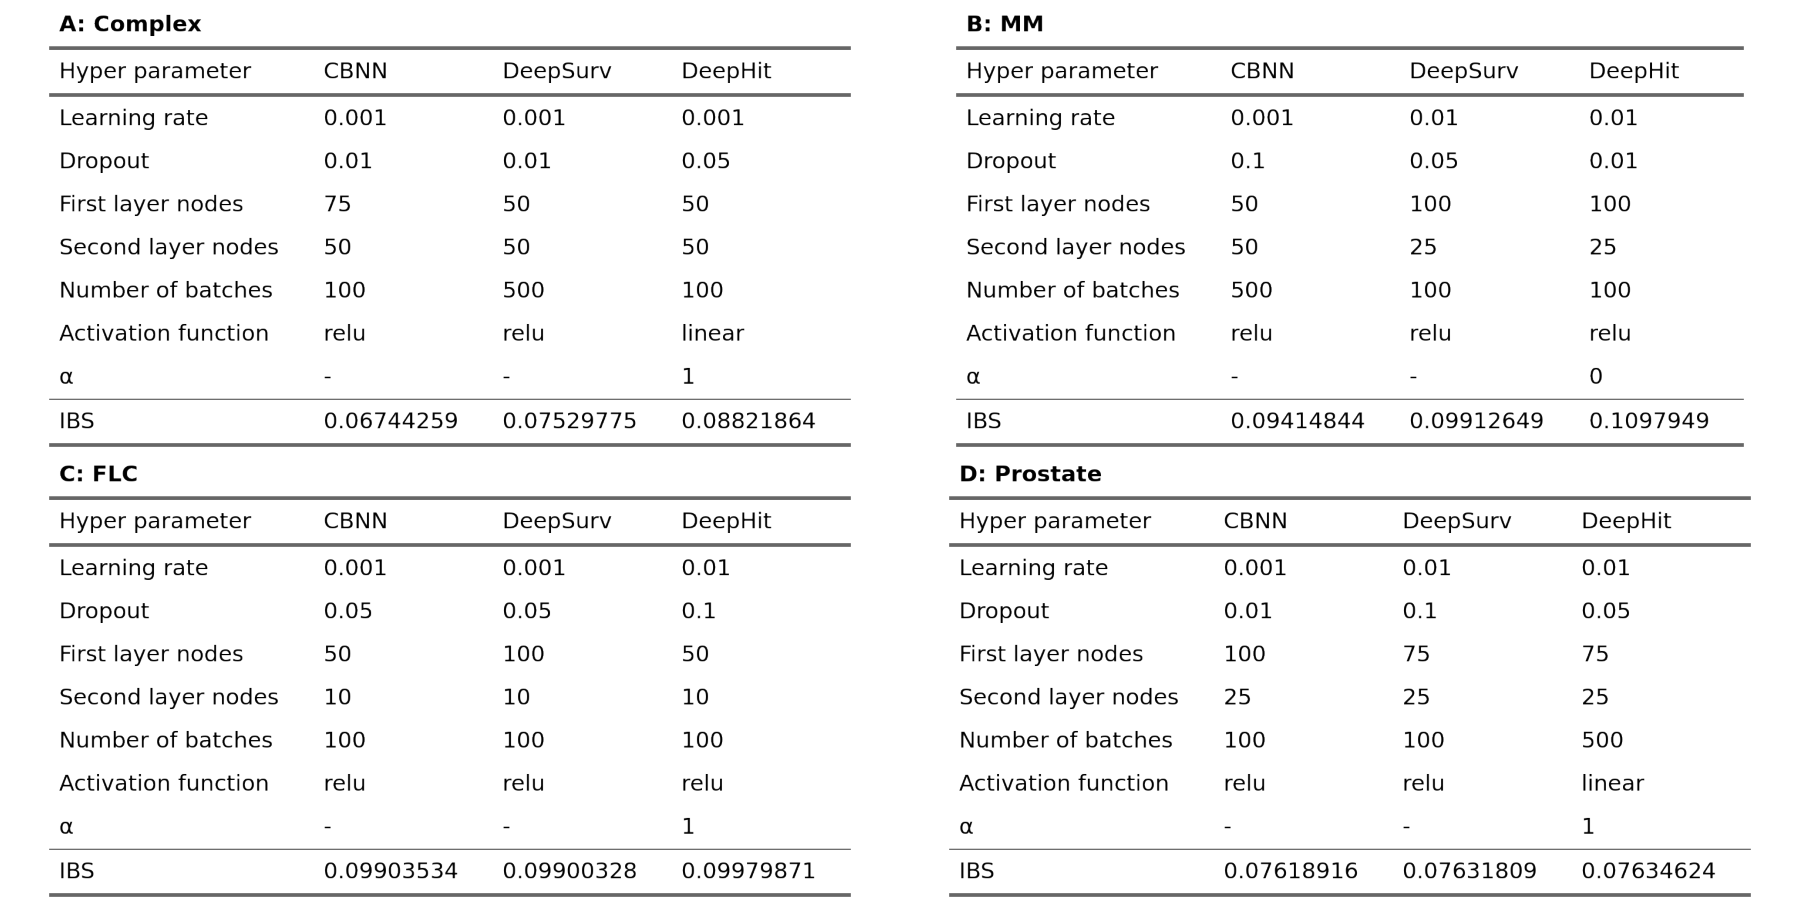
\includegraphics[width=1\linewidth]{../figures/winTable} \end{center}
\end{table}

DeepHit uses $\alpha$ as a specific hyperparameter, while DeepSurv and CBNN do not.
We track IBS on the validation set for each hyperparameter combination,
choosing the combination with the lowest score for each method.
We present the chosen hyperparameters in Table 1.

\hypertarget{software-implementation}{%
\subsection{Software implementation}\label{software-implementation}}

R \citep{Rsoft} and python \citep{py} are used to evaluate methods from
both languages. We fit the Cox model using the \textbf{survival} package
\citep{survpkg}, the CBLR model using the \textbf{casebase} package
\citep{cbpkg}, DeepSurv and DeepHit using \textbf{pycox}
\citep{lee2018DeepHit}. We made the components
of CBNN using the \textbf{casebase} package for the sampling step and
the \textbf{keras} \citep{keras} package for our neural network
architecture. The \textbf{simsurv} package \citep{simsurv} is used for
our simulation studies, while \textbf{flexsurv} \citep{flexsurv} is used
to fit a flexible baseline hazard using splines for our complex
simulation. The \textbf{riskRegression}
package \citep{riskRegression} is used to get the Index of Prediction
Accuracy (IPA metric) and AUC. Both metrics are described in detail in the
following section. We modify the \textbf{riskRegression} package to be
used with any user supplied risk function \(F\). To ensure that both R
and Python-based models are running in unison on the same data through
our simulations and bootstrap, we use the \textbf{reticulate} package
\citep{reticulate}.



%%%%%%%%%%%%%%%%%%%%%%%%%%%%%%%%%%%%%%%%%%%%%%
%%%%%%%%%%%%%%%%%%%%%%%%%%%%%%%%%%%%%%%%%%%%%%
%%%%%%%%section3
%%%%%%%%%%%%%%%%%%%%%%%%%%%%%%%%%%%%%%%%%%%%%%
%%%%%%%%%%%%%%%%%%%%%%%%%%%%%%%%%%%%%%%%%%%%%%



\begin{figure}

{\centering 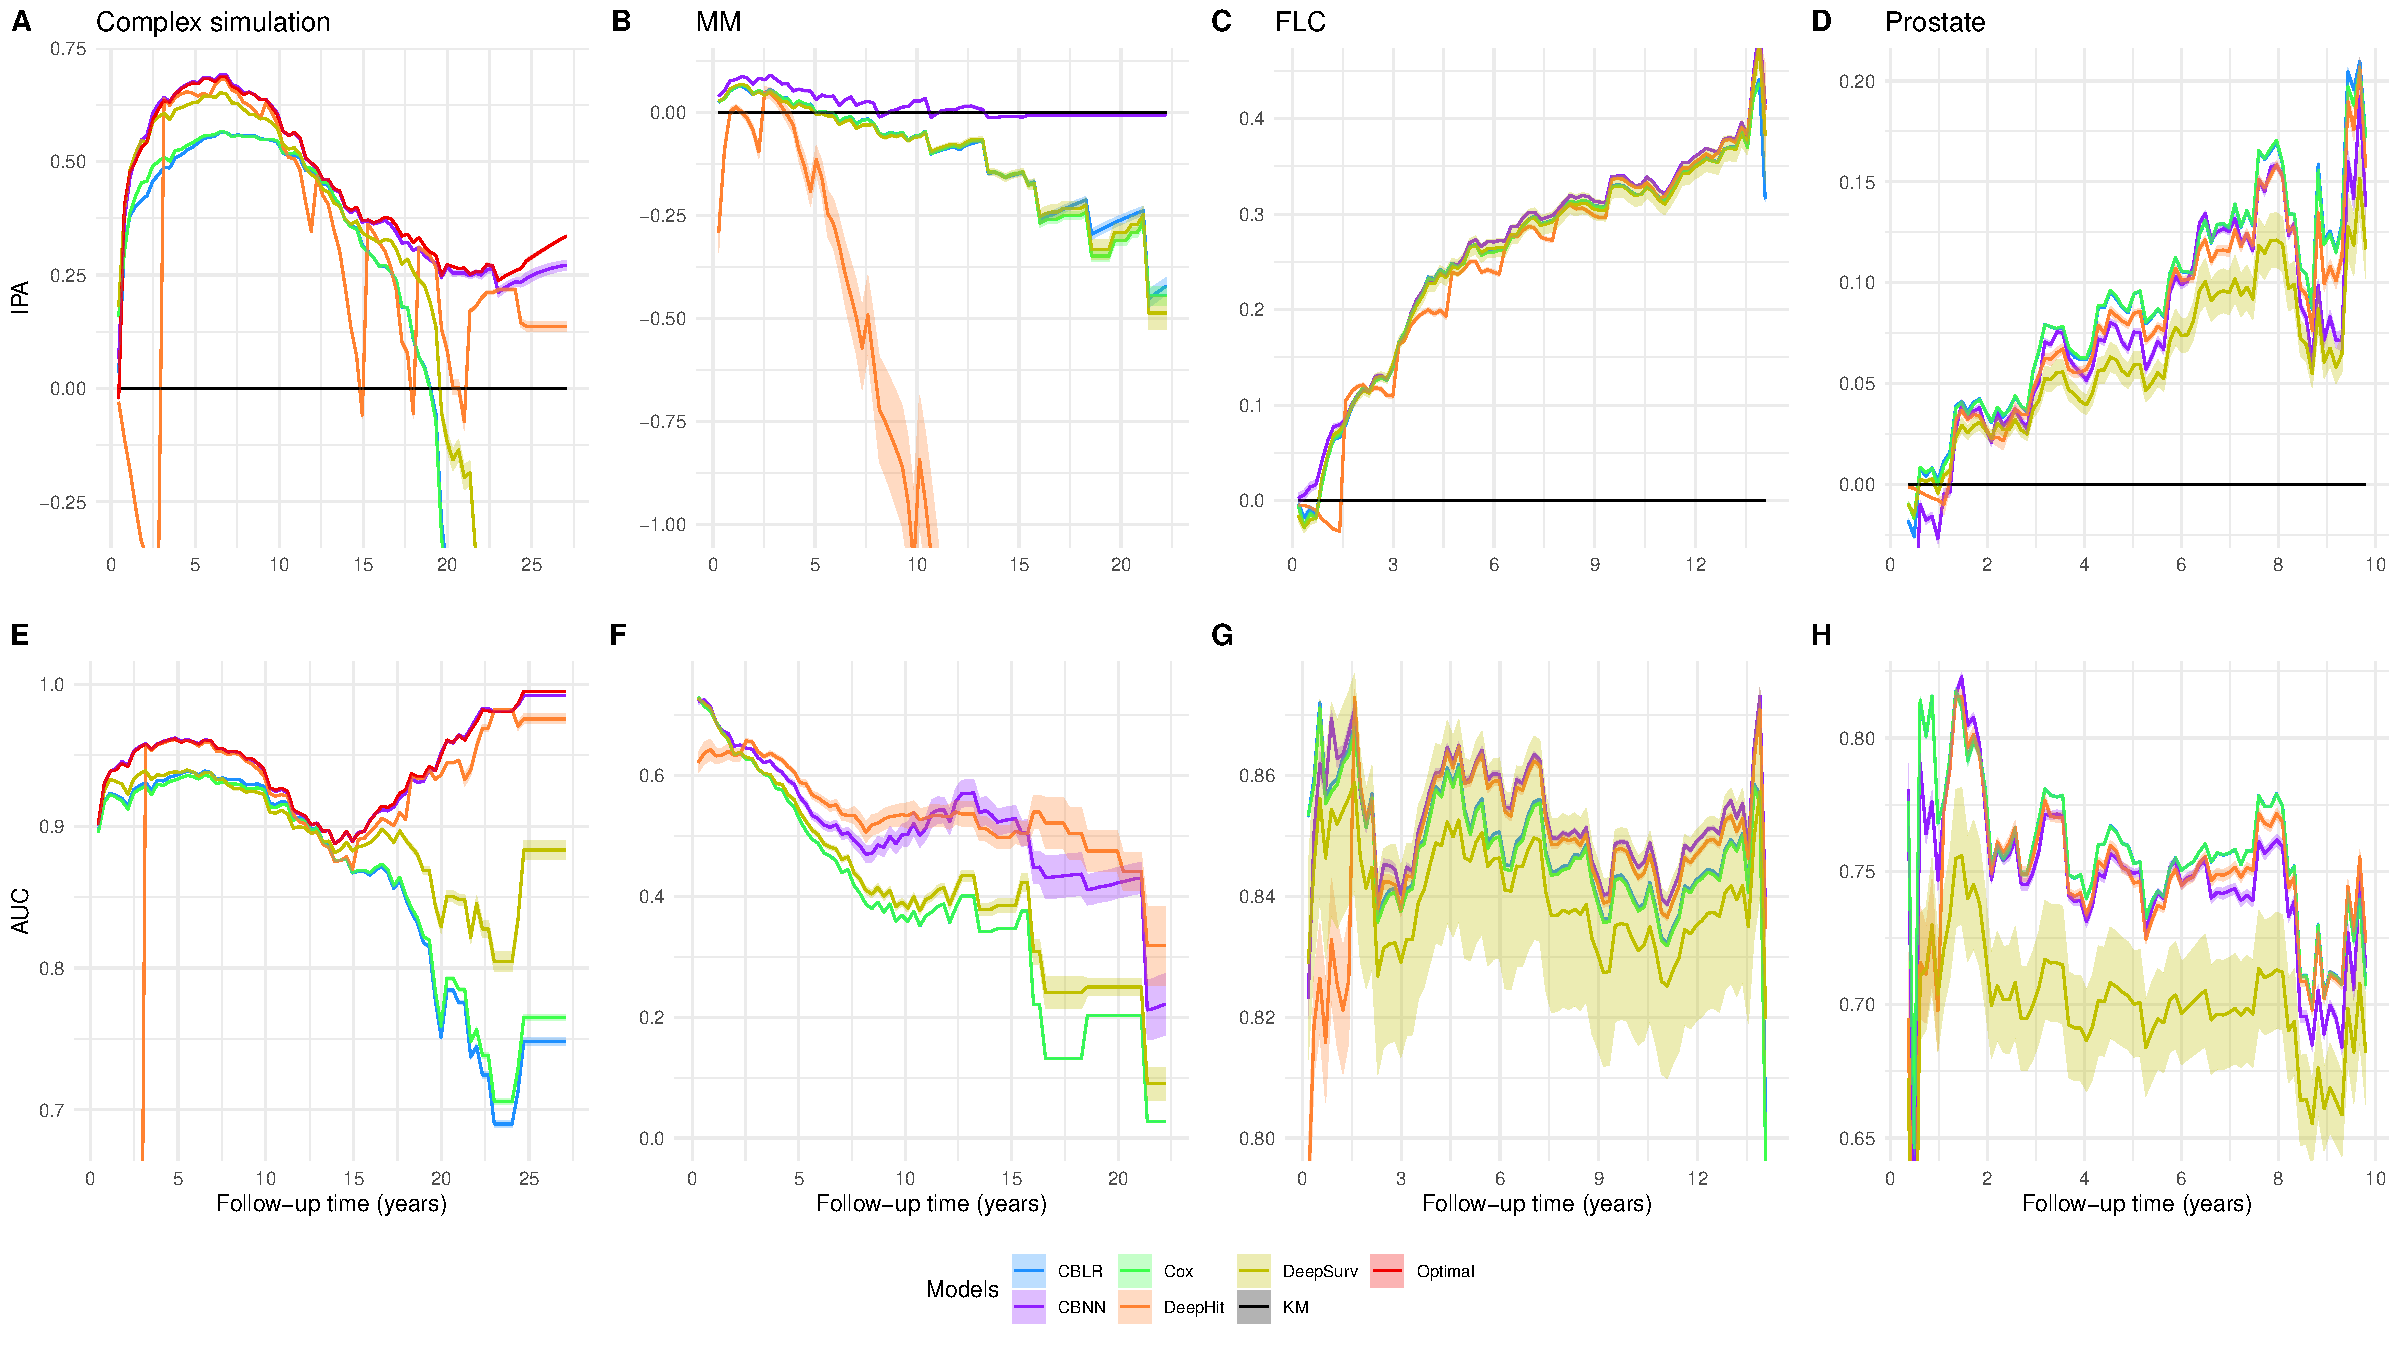
\includegraphics[width=1\linewidth]{../figures/megaPlot} 

}

\caption{Summarizes the complex simulation (A, E), multiple myeloma (MM) case study (B, F), free light chain (FLC) case study (C, G) and prostate cancer (Prostate) case study (D, H). The first row shows the IPA for each model in each study over follow-up time. Negative values mean our model performs worse than the null model and positive values mean the model performs better. The second row shows the $AUC_{IPCW}$ for each model in each study over follow-up time. Each model-specific metric in each study shows a 95\% confidence interval over 100 iterations. The models of interest are case-base with logistic regression (CBLR), Case-Base Neural Networks (CBNN), Cox, DeepHit and DeepSurv. Both CBLR and Cox have near identical performance, resulting in curves that are overlapped. The Kaplan-Meier (KM) model serves as a baseline, predicting the average curve for all individuals. The Optimal (a CBLR model with the exact interaction terms and baseline hazard specified) model shows the best performance we can expect on the simulated data. }\label{fig:megaPlot}
\end{figure}



\hypertarget{sims}{%
\section{Simulation study}\label{sims}}

In this section, we simulate data to evaluate the performance of
CBNN and compare our approach with existing regression-based (Cox, CBLR)
and neural network-based (DeepHit, DeepSurv) methods. We specify a
linear combination of each covariate as the linear predictor in
regression-based approaches (Cox, CBLR), which contrasts with neural
network approaches that allow for non-linear interactions. We simulate
data under a complex baseline hazard with
time-varying interactions, each with 10\% random censoring. For both
settings, we simulate three covariates for 5000 individuals:

\[
z_{1} \sim \textrm{Bernoulli}(0.5) \qquad \qquad %technically a control and treatement group
z_{2} \sim \begin{cases}
 N(0,0.5) & \textrm{if } z_{1}=0\\ 
 N(1,0.5) & \textrm{if } z_{1}=1
\end{cases} \qquad \qquad
z_{3} \sim N(1,0.5).
\]
Besides the methods mentioned above, we include the Optimal model in our comparisons using CBLR.
We include the exact functional form of the covariates in a CBLR model (referred to as Optimal for simplicity).
We conduct 100 bootstrap re-samples on the training data to get confidence intervals. We kept 15\% of the
data for testing before hyperparameter selection. 15\% of the remaining data is used for validation and the rest is reserved
for training. We predict risk functions for individuals in the test set, which are used to calculate our $AUC_{IPCW}$ and IPA. 





\hypertarget{complex-simulation-flexible-baseline-hazard-time-varying-interactions}{%
\subsection{Complex simulation: flexible baseline hazard, time-varying
interactions}\label{complex-simulation-flexible-baseline-hazard-time-varying-interactions}}

This simulation shows performance with the presence of a complex
baseline hazard and a time-varying interaction. Inspired by a cancer treatment
that initially reduces risk of death, but slowly returns as time progresses. 
Originally used to show the spline-based hazard model proposed by Royston and Parmar
\citep{royston2002flexible}, the breast cancer dataset provides a
complex baseline hazard from which we simulate, available in the
\textbf{flexsurv} R package \citep{flexsurv}. To increase the complexity
of our data-generating mechanism for this simulation, we design the
model \begin{align}
\log h(t \mid X_i) =\sum_{i=1}^{5} (\gamma_{i} \cdot \psi_{i}) + \beta_{{1}} (z_{1}) + \beta_{{2}} (z_{2})+ \beta_{{3}} (z_{3})+ \tau_{1} ( z_{1} \cdot t)+ \tau_{2} (z_{2} \cdot z_{3}), \nonumber
\end{align}




where
\(\gamma_{1}=3.9, \gamma_{2}=3, \gamma_{3}=-0.43, \gamma_{4}=1.33,\gamma_{5}=-0.86, \beta_{{1}}=-5, \beta_{{2}}=-1, \beta_{{3}}=1, \tau_{1}=0.001, \tau_{2}=-1\)
and \(\psi\) are basis splines. The \(gamma\) coefficients are obtained
from an intercept-only cubic splines model with three knots using the
\emph{flexsurvspline} function from the \textbf{flexsurv} package
\citep{flexsurv}. Note that we fix these values for the analysis. The
\(\beta\) coefficients represent direct effects, \(\tau_{2}\) represents
an interaction and \(\tau_{1}\) is a time-varying
interaction.

\hypertarget{performance-comparison-in-complex-simulation}{%
\subsection{Performance comparison in complex
simulation}\label{performance-comparison-in-complex-simulation}}


Figure \ref{fig:megaPlot} A, E and Table \ref{tab:megaTable} A
shows the performance over time on a test set. For discrimination, the Optimal model
performs best as expected, followed by CBNN, DeepHit, DeepSurv and the linear models (Figure \ref{fig:megaPlot} E).
For both discrimination and calibration, the rankings remain the same aside from DeepHit,
where there's a periodic loss in performance (Figure \ref{fig:megaPlot} A). The
Optimal model acts as a reference for how good a model can perform,
with CBNN performing better than the competitors in the complex simulation.
To obtain a more realistic performance assessment, we compared models in
three case studies with a time-to-event outcome.


\begin{table}[!htbp]
\caption{Four tables representing performance at certain percentages of follow-up time in the complex simulation (A), multiple myeloma (MM) case study (B), free light chain (FLC) case study (C) and prostate cancer (Prostate) case study (D). Each table shows performance for each method in each study at $25\%$, $50\%$. $75\%$ and $100\%$ of follow-up time. The bold elements show the best model for each study, at each follow-up time of interest. These tables are included to provide exact measures at certain intervals. The models of interest are: Cox, case-base with logistic regression (CBLR), DeepSurv, DeepHit, Case-Base Neural Network (CBNN) and Optimal (in the complex simulation). The CBNN label is in bold to make it easier to distinguish. The best score at each percent of follow-up time is highlighted in bold. If the average performance is tied, then all tied values are bold.}
\label{tab:megaTable}

\begin{center}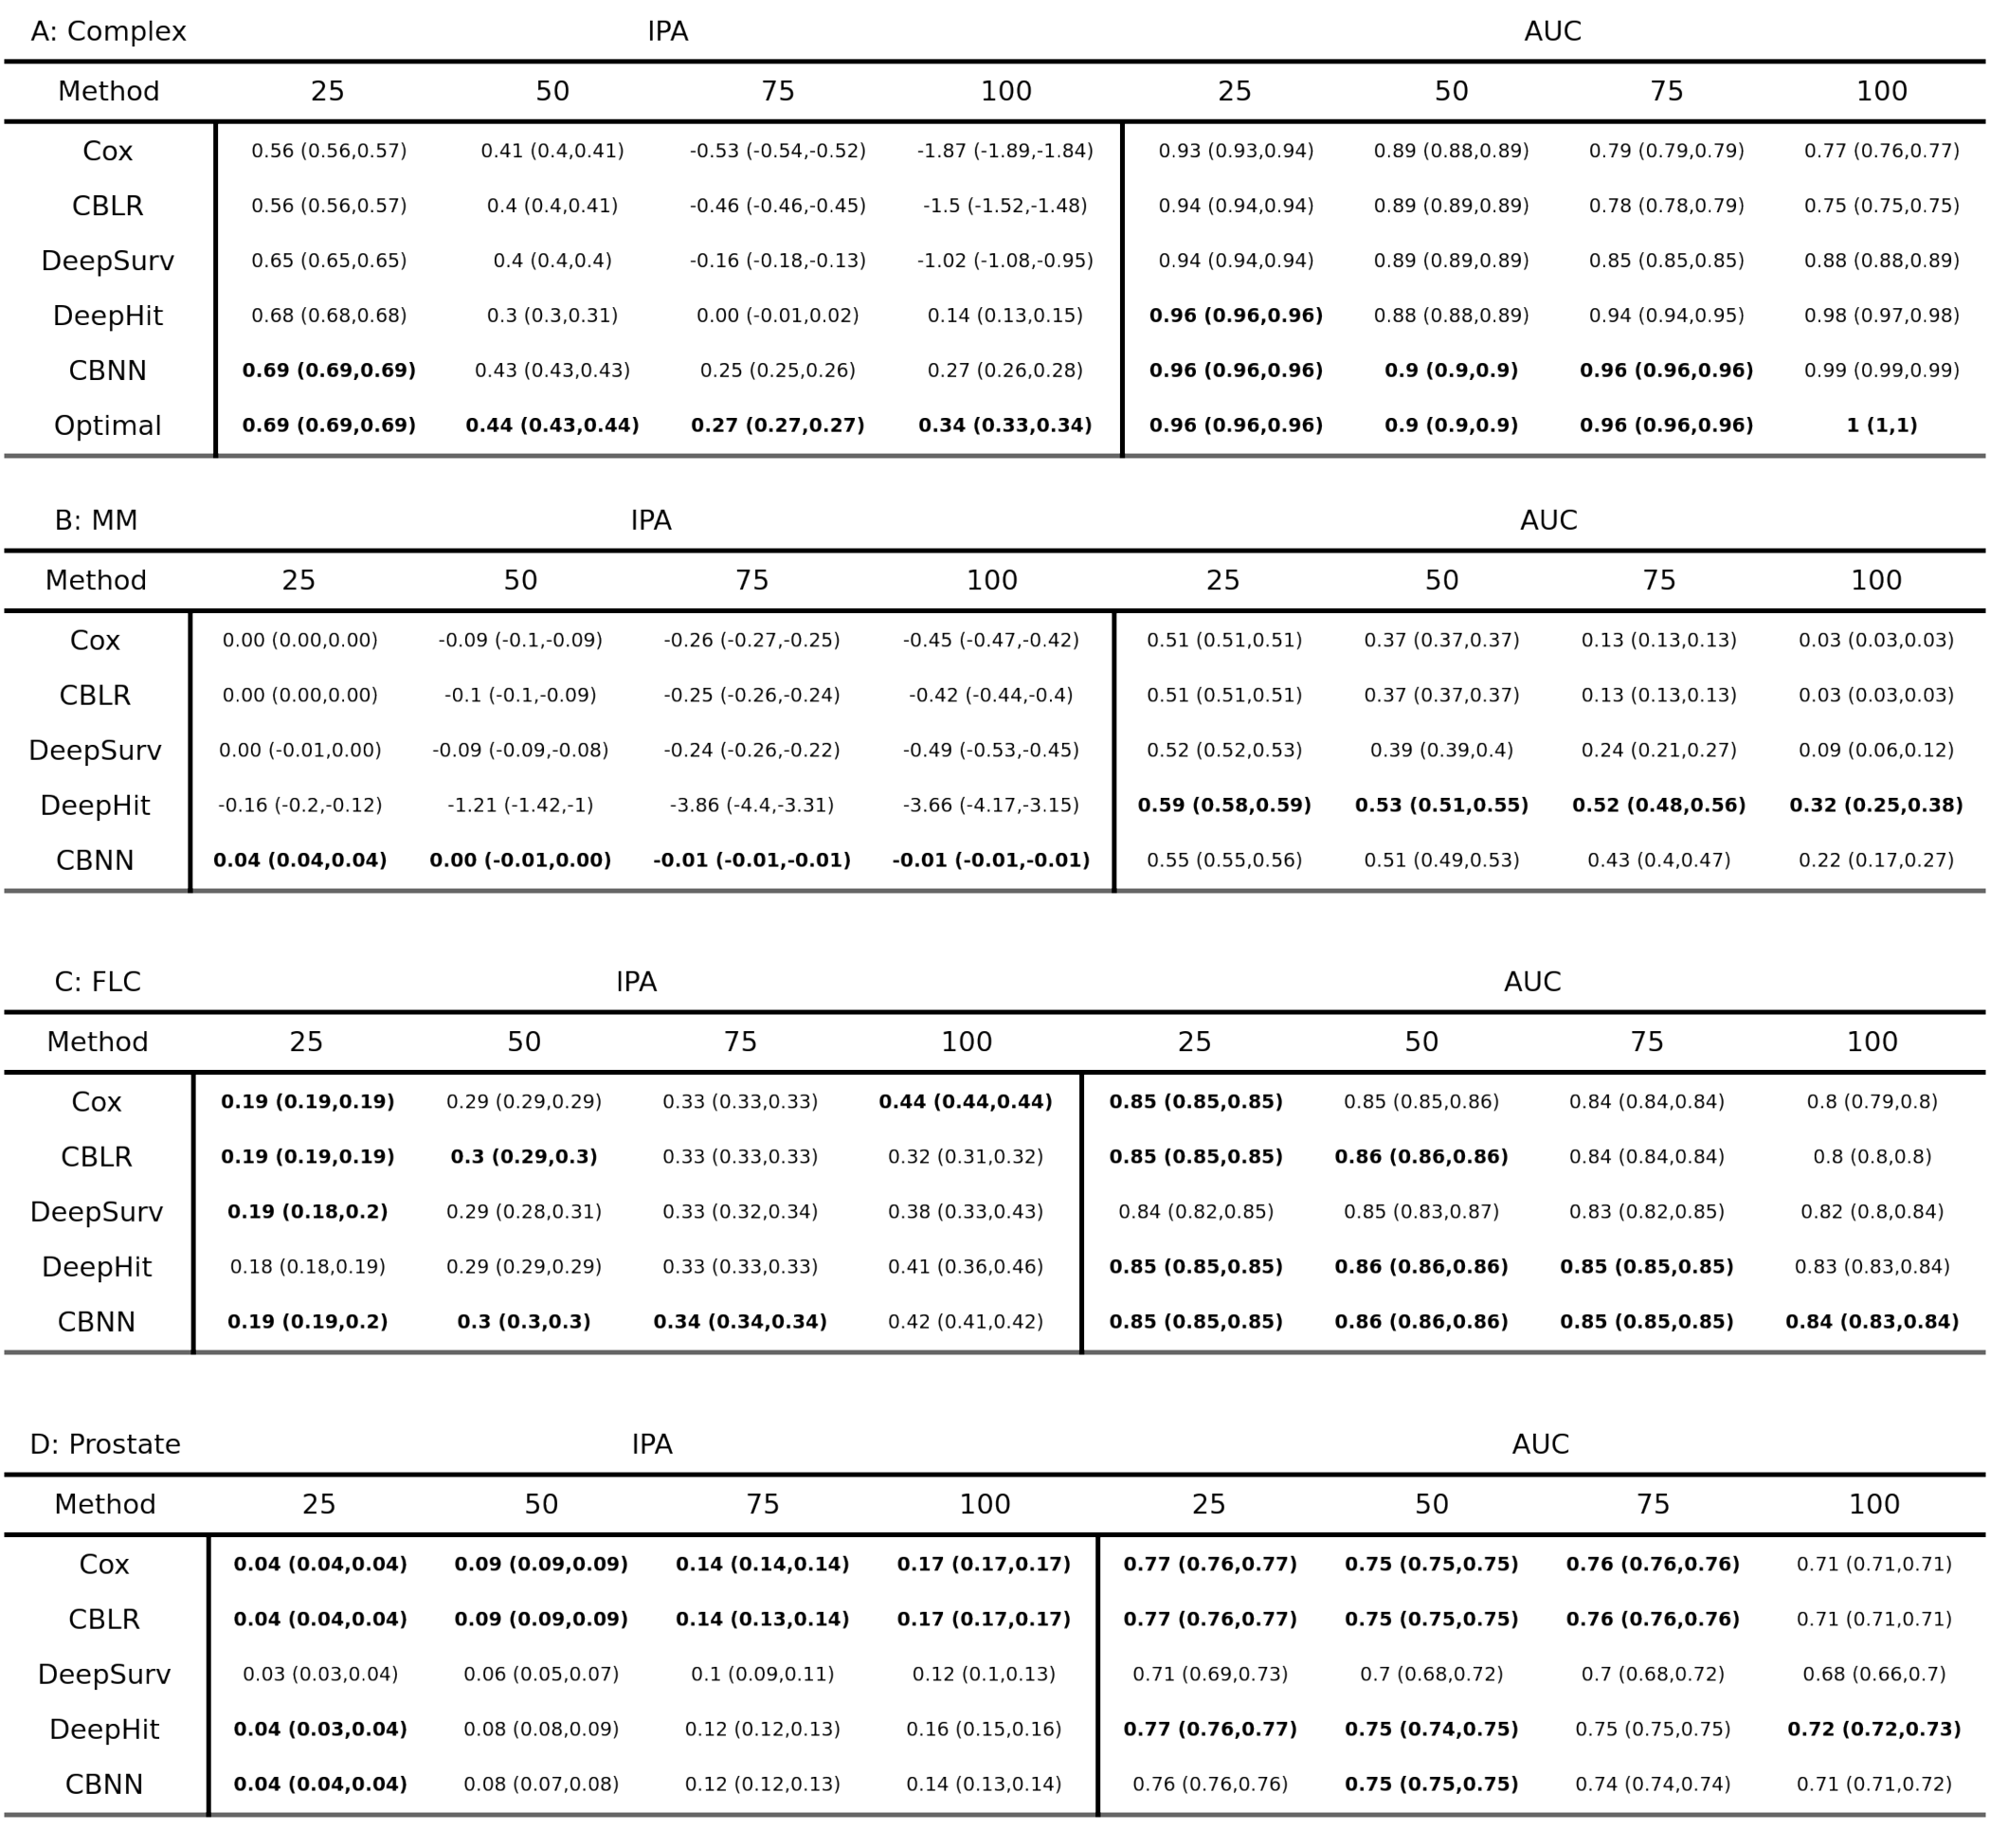
\includegraphics[width=1\linewidth]{../figures/megaTable} \end{center}

\end{table}

%%%%%%%%%%%%%%%%%%%%%%%%%%%%%%%%%%%%%%%%%%%%%%
%%%%%%%%%%%%%%%%%%%%%%%%%%%%%%%%%%%%%%%%%%%%%%
%%%%%%%%section4
%%%%%%%%%%%%%%%%%%%%%%%%%%%%%%%%%%%%%%%%%%%%%%
%%%%%%%%%%%%%%%%%%%%%%%%%%%%%%%%%%%%%%%%%%%%%%


\hypertarget{casestudies}{%
\section{Casestudies}\label{casestudies}}

 The first case study examines multiple myeloma (MM) \citep{myeloma}.
Case study two examines the relationship between serum free light chain (FLC) and mortality \citep{flc}.
The third examines prostate cancer (Prostate) survival on a publicly available simulation of the Surveillance,
Epidemiology, and End Results (SEER)-medicare study \citep{prostate}. Both MM and FLC
are available as part of the \textbf{survival} package \citep{survpkg}. The Prostate dataset is available
as part of the \textbf{asaur} package \citep{asaur}. As we do not know the true model for the case studies,
we exclude the Optimal model. After we perform grid search with the same hyperparameter
options, we split the data the same way we did for the simulation (allocated 15\% of the data for testing,
15\% of the remaining data for validation, and the rest for testing).
We predict risk functions for everyone in the test set, which is used to calculate our metrics. We
conduct 100-fold bootstrap re-samples on the training data to
get confidence intervals.

\hypertarget{pe-multiplemyeloma}{%
\subsection{Performance evaluation on multiple myeloma dataset}\label{pe-multiplemyeloma}}
The MM study tracks 3882 patients seen at the Mayo Clinic from 1947 to 1996 until death \citep{myeloma}.
We use 2 covariates, year of entry into the study and the time of MM diagnosis\citep{myeloma}.
We see 71\% incidence over 23 years\citep{myeloma}.

Figure \ref{fig:megaPlot} B, F and Table \ref{tab:megaTable} B
demonstrate the performance over time on a test set. For discrimination,
CBNN and DeepHit have a similar performance, followed by DeepSurv and finally the linear models performing worst (Figure \ref{fig:megaPlot} F). For
both discrimination and calibration, CBNN performs substantially better than
the linear models and DeepSurv, with DeepHit having the worst performance overall
(Figure \ref{fig:megaPlot} B). Together, CBNN is the best calibrated model and one
of the best at discrimination in the MM case study.

%paragraph about performance

\hypertarget{pe-flc}{%
\subsection{Performance evaluation on free light chain dataset}\label{pe-flc}}
The FLC dataset is a random sample of half the individuals in $\frac{2}{3}$ of the
residents of Olmsted County over the age of 50 \citep{flc}. We have access to 7874 subjects
tracked until death \citep{flc}. We use 5 covariates, total serum FLC (sum of kappa and lambda), age, sex,
serum creatine and monoclonal gammapothy state \citep{flc}. There is 27\% incidence over 14 years \citep{flc}.

Figure \ref{fig:megaPlot} C, G and Table \ref{tab:megaTable} C
demonstrate the performance over time on a test set. CBNN, DeepHit and the linear models
perform best at discrimination, followed DeepSurv (Figure \ref{fig:megaPlot} G). The rankings
remain the same aside from DeepHit where the performance periodically drops
to worse than DeepSurv (Figure \ref{fig:megaPlot} C). Together, CBNN outperforms the competing models,
in terms of both calibration and discrimination in the FLC study. However, CBNN is only slightly better
than the linear ones.

\hypertarget{pe-prostate}{%
\subsection{Performance evaluation on prostate cancer dataset}\label{pe-prostate}}
The prostate cancer dataset has a record of competing risks \citep{prostate}. As we are only interested in the
single event scenario, we only keep individuals with prostate cancer death or censoring \citep{prostate}.
This subset tracks 11054 individuals with three covariates: differentiation grade, age group and cancer state \citep{prostate}.
There is a 7\% incidence over 10 years.

Figure \ref{fig:megaPlot} C, G and Table \ref{tab:megaTable} C demonstrate the
performance over time on a test set. In the prostate case study, the linear models
outperform the other models in both discrimination and calibration, followed by
CBNN and DeepHit and finally DeepSurv (Figure \ref{fig:megaPlot} C, G). Aside from DeepSurv,
the performance is similar across all models.


%%%%%%%%%%%%%%%%%%%%%%%%%%%%%%%%%%%%%%%%%%%%%%
%%%%%%%%%%%%%%%%%%%%%%%%%%%%%%%%%%%%%%%%%%%%%%
%%%%%%%%section6
%%%%%%%%%%%%%%%%%%%%%%%%%%%%%%%%%%%%%%%%%%%%%%
%%%%%%%%%%%%%%%%%%%%%%%%%%%%%%%%%%%%%%%%%%%%%%


\hypertarget{discussion}{%
\section{Discussion}\label{discussion}}

CBNN models survival outcomes by using neural networks on case-base
sampled data. We incorporate follow-up time as a feature, providing a
data-driven estimate of a flexible baseline hazard and time-varying
interactions in our hazard function. The two competing neural network
models we evaluated cannot model time-varying interactions
 \citep{katzman2018DeepSurv} \citep{lee2018DeepHit}.
 
A method we want to include is Deep Survival Machines (DSM), a
parametric survival model using neural networks with a mixture of
distributions as the baseline hazard \citep{dsmPaper}. It can model
a flexible baseline hazard. However, like DeepHit
and DeepSurv, DSM cannot model time-varying interactions \citep{dsmPaper}. DSM
requires a two-phase learning process and user implementations for
distributions beyond Log-Normal or Weibull
\citep{dsmPaper}. DSM outperformed DeepSurv and DeepHit, but only tested
a subset of hyperparameter combinations for competing neural network methods
while going through a full grid search for their method \citep{dsmPaper}.
With our hyperparameters options and model design, DSM did not
converge in the complex simulation. This may be due to implementation issues or
method limitations, therefore we did not include this method.

Compared to CBNN, the neural network competitors also have limitations.
DeepSurv is a proportional hazards model and does
not estimate the baseline hazard \citep{katzman2018DeepSurv}. DeepHit
requires an alpha hyperparameter, assumes a single distribution
for the baseline hazard and models the survival function directly
\citep{lee2018DeepHit}. The alternative neural network methods
match on time, while CBNN models time directly.

Though we applied a full grid search for all neural network models,
there are an infinite number of untested hyperparameters we did not
test. A completely exhaustive search is computationally infeasible,
therefore it is reasonable to expect that there is a set of hyperparameters
that is better suited for each model. However, we test a reasonably large
range while accounting for potential over-fitting by including dropout
\citep{gulli2017}. We provided the same options to all models aside from
DeepHit, which has a method specific hyperparameter $\alpha$
\citep{lee2018DeepHit}. With these limitations in mind, we dive
into the differences in performance across all tested methods.

The complex simulation requires a method that can learn both time-varying
interactions and have a flexible baseline hazard. Here, CBNN shows
a distinct advantage over all other methods. Based on our complex simulation results (Figure
\ref{fig:megaPlot} A, E and Table \ref{tab:megaTable} A), CBNN
outperforms the competitors. This simulation shows how all models perform
under ideal conditions with minimal noise in the data, while the three case studies
assess their performance in realistic conditions. In the MM case study, flexibility in both
interaction modeling and baseline hazard improves CBNN's performance over
the other models, suggesting that this flexibility aids calibration (Figure
\ref{fig:megaPlot} B, F and Table \ref{tab:megaTable} B). upon examination of the FLC case study,
CBNN demonstrates small improvement to performance compared to the linear models and DeepHit
for both IPA and AUC (Figure \ref{fig:megaPlot} C, G and Table \ref{tab:megaTable} C).
In the Prostate case study, the linear models outperform
the neural network ones, while CBNN and DeepHit alternate their positions depending
on the follow-up time of interest and DeepSurv maintains last place
(Figure \ref{fig:megaPlot} C, G and Table \ref{tab:megaTable} C). We attribute this to
potential over-parameterization in the neural network models, as we did not test for fewer
nodes in each hidden layer, even with dropout. Though the
ranking places the linear models above the neural network ones, the overall
performance is comparable aside from DeepSurv, falling within a small range of IPA and AUC values.

If prediction is our goal, we suggest CBNN as the best model in the Complex simulation, MM case study
and FLC case study. The linear models were competitive in the FLC case study and performed best
in the prostate case study. Though neural network interpretability is steadily improving \citep{interpret},
there is still a trade-off compared to regression models, especially
when the predictive performance gain is minimal, like in the FLC case study. We suggest that reference models should be included
when assessing neural network models. Both a null model (KM curve) and a linear model (either Cox or
a flexible baseline hazard model like CBLR) provide insight as to whether the neural network model is learning
anything useful beyond linear predictors that were not accounted for.

\section{Conclusions}\label{sec5}

CBNN outperforms all competitors in the complex
simulation and two case studies while maintaining competitive performance in a final case study.
Once we perform case-base sampling and adjust for the sampling bias, we can use
a sigmoid activation function to predict our hazard function. Our
approach provides an alternative to incorporating censored individuals, treating
survival outcomes as binary ones. Forgoing the requirement
of custom loss functions, CBNN only requires the use of standard
components in machine learning libraries (specifically, the add layer to
adjust for sampling bias and the sigmoid activation function) after case-base sampling. Due to
the simplicity in its implementation and by extension user experience,
CBNN is both a user-friendly approach to data-driven survival analysis
and is easily extendable to any feed-forward neural network framework.

%\backmatter

\hypertarget{data-and-code-availability-statement}{%
\subsection*{Data and code availability
statement}\label{data-and-code-availability-statement}}
\addcontentsline{toc}{section}{Data and code availability statement}


The Prostate dataset is available as part of the \textbf{asaur} package in R.
The MM and FLC datasets are available in the \textbf{survival} package in R.
The code for this manuscript and its analyses can be found at
\url{https://github.com/Jesse-Islam/cbnnManuscript}. The software
package making CBNN easier to implement can be found at
\url{https://github.com/Jesse-Islam/cbnn}.

\hypertarget{acknowledgements}{%
\subsection*{Acknowledgements}\label{acknowledgements}}
\addcontentsline{toc}{section}{Acknowledgements}

We would like to thank Dr.~James Meigs, the project
leader of these awards, for his support and helpful discussions. The
work was also supported as part of the Congressionally Directed Medical
Research Programs (CDMRP) award W81XWH-17-1-0347. We would also like to
thank Dr.~James Hanley for his support and discussions while extending
the case-base methodology.

\subsection*{Author contributions}

J.I. conceived the proof of concept, developed the theoretical formalism, developed the neural network code base, wrote the majority of the manuscript and performed the simulations and analyses. M.T. wrote the majority of the casebase sampling section \ref{case-base-sampling}. M.T. and S.B. provided key insights into the core sampling technique (casebase). R.S. provided multiple edits to the manuscript structure and key insights. All authors discussed the results and contributed to the final manuscript.

\subsection*{Financial disclosure}

This work was supported by subcontracts from UM1DK078616 and R01HL151855
to Dr.~Rob Sladek. 

\subsection*{Conflict of interest}

The authors declare no potential conflict of interests.


\appendix
%\nocite{*}% Show all bib entries - both cited and uncited; comment this line to view only cited bib entries;
\bibliography{wileyNJD-APA}%


\section*{Author Biography}

\begin{biography}{
\includegraphics[width=60pt,height=70pt,draft]{empty}}{\textbf{Jesse Islam} A PhD Candidate in Quantitative life sciences, studying complex relationships in data in a survival context.}
\end{biography}

\end{document}
